% =====================================================================
%  diagnostico_miranda.tex -- Documento de trabajo para el autor.
%  Diagnostico de las observaciones del Ing. Julio Saul Miranda
%  (tribunal), transmitidas por el autor el 2026-09-25, y como se
%  aplicaron en la version final3 de la tesis (main_final3.tex).
%  Fuentes: las tres presentaciones de Miranda y los Talleres 1-6 de
%  Barrios (tesis/Material docente/), la version final2 y final3.
%  Compilar: pdflatex diagnostico_miranda  (dos veces, por las referencias)
%  NO forma parte de la tesis.
% =====================================================================
\documentclass[11pt,a4paper]{article}
\usepackage[utf8]{inputenc}
\usepackage[T1]{fontenc}
\usepackage{lmodern}
\usepackage[spanish,es-tabla]{babel}
\usepackage[a4paper,margin=2.2cm]{geometry}
\usepackage{booktabs,array,longtable}
\usepackage{xcolor}
\usepackage{enumitem}
\usepackage{graphicx}
\graphicspath{{../capitulos_final3/figuras/}}
\usepackage[hidelinks]{hyperref}
\usepackage{amsmath}
\setlength{\parskip}{5pt}
\setlength{\parindent}{0pt}
\setlength{\tabcolsep}{4pt}
\setlist{itemsep=2pt,topsep=3pt}
\newcolumntype{L}[1]{>{\raggedright\arraybackslash}p{#1}}
\AtBeginDocument{\DeclareRobustCommand{\%}{\char37\relax}}
\newcommand{\enunciado}[1]{\begin{center}\fbox{\parbox{0.93\textwidth}{\raggedright #1}}\end{center}}
\definecolor{adopta}{HTML}{198754}
\definecolor{adapta}{HTML}{B35C00}
\newcommand{\adopta}{\textcolor{adopta}{\textbf{Se adopta}}}
\newcommand{\adapta}{\textcolor{adapta}{\textbf{Se adopta con ajustes}}}

\title{Observaciones del Ing.\ Miranda: diagnóstico y aplicación\\
\large Qué se adoptó, qué se ajustó y por qué, en la versión \texttt{final3} de la tesis}
\author{Documento de trabajo para el autor}
\date{25 de septiembre de 2026}

\begin{document}
\maketitle

\section*{La decisión, en una página}

El Ing.\ Julio Saúl Miranda revisó la tesis con rapidez y dejó nueve observaciones sobre la causa y el efecto, el problema, el objetivo general, los objetivos específicos, la hipótesis, las conclusiones y el formato. No son mandatos, y algunas estaban dichas de prisa: repetían un verbo en dos capítulos o usaban un absoluto que la propia tesis refuta. Por eso cada una se contrastó con sus propias láminas, con los talleres de la Carrera y con el contenido de la tesis antes de aplicarla.

\textbf{Resultado: las nueve se adoptan en su fondo.} En cinco se ajusta la forma, siempre con un motivo que se puede sostener frente a él:
\begin{itemize}
    \item el problema conserva el molde de su propia lámina (\emph{«¿De qué manera\ldots{} podrá incidir en\ldots?»}) en lugar de \emph{«¿Cómo\ldots{} genera\ldots?»};
    \item \emph{«escasa»} transparencia en lugar de \emph{«nula»}, porque la Tabla 1.1 de la tesis dice «Baja (caja negra)»;
    \item \emph{«procedimiento de cálculo»} en lugar de \emph{«proceso interno»}, el término canónico de la tesis;
    \item el objetivo general se completa con el \emph{¿cómo?} que su lámina exige y que la sugerencia omitía;
    \item «verificar», que la sugerencia repartía entre dos capítulos, queda solo en el Capítulo 3.
\end{itemize}

Todo se aplicó en una versión nueva, \textbf{final3} (\texttt{main\_final3.tex} y \texttt{capitulos\_final3/}). \textbf{Este trabajo no modificó final2}, que queda como base de comparación; solo recibió, aparte, el retiro de PyMuPDF que otra sesión aplicó a pedido del autor. La formulación queda así:

\enunciado{\textbf{Problema.} ¿De qué manera la escasa transparencia del procedimiento de cálculo del software de análisis por elementos finitos podrá incidir en la baja trazabilidad y verificabilidad de ese procedimiento, en la gestión 2026?}

\enunciado{\textbf{Objetivo general.} Desarrollar un software educativo de elementos finitos para el análisis estructural, empleando el lenguaje de programación Python, debido a la escasa transparencia del procedimiento de cálculo del software de análisis, para mejorar la trazabilidad y la verificabilidad del procedimiento de cálculo.}

\enunciado{\textbf{Hipótesis.} El desarrollo de EduFEM permitirá mejorar la transparencia del procedimiento de cálculo por elementos finitos ---de caja negra a procedimiento a la vista---, elevando su trazabilidad y su verificabilidad.}

Los objetivos específicos pasan de cinco a \textbf{tres, uno por capítulo}: \emph{Fundamentar}, \emph{Desarrollar}, y \emph{Verificar y validar}. Cada objetivo, completo, es el título de su capítulo. «Diagnosticar» deja de ser objetivo y su contenido pasa a la fundamentación. Las conclusiones siguen la \emph{tríada} de su lámina (capítulo, conclusión, recomendación), con dos figuras y una tabla. El texto va en Times New Roman 12 y justificado.

\section{Las nueve observaciones, una por una}

Las láminas se citan así: \textbf{PP} = \emph{Planteamiento del problema científico e hipótesis}; \textbf{OG} = \emph{Cómo se construye el objetivo general}; \textbf{SP} = \emph{Situación problemática, objeto de estudio y campo de acción} (las tres de Miranda); \textbf{T1\ldots T6} = Talleres de Barrios. El número que sigue es el de la lámina.

\subsection*{1. Causa y efecto}
\textbf{Lo que dijo.} Causa: la transparencia, la exposición del procedimiento de cálculo interior del software. Efecto: la trazabilidad y la verificabilidad del proceso interno.\\
\textbf{Veredicto.} \adapta{} (solo términos).\\
\textbf{Por qué.} Es la misma relación que la tesis ya tenía, dicha con más nitidez. Se cambian dos palabras:
\begin{itemize}
    \item «transparencia, exposición» son dos nombres para lo mismo. La variable se llama \emph{transparencia del procedimiento de cálculo}, y «exposición» pasa a su definición: \emph{la exposición que el software hace de su procedimiento de cálculo interno}.
    \item «proceso interno» pasa a \emph{procedimiento de cálculo}, el término que la tesis fija y define, que además evita «proceso de cálculo».
\end{itemize}
Hay además una mejora de fondo: causa y efecto quedan como \emph{atributos de la unidad de análisis} que declara el §2.1.4 (el procedimiento de cálculo). Es lo que pide PP 5 («las variables son los aspectos del objeto de estudio que serán medidos») y lo que muestra su ejemplo: diseño de la losa → costo de la losa, dos atributos del mismo objeto.

\subsection*{2. El problema}
\textbf{Lo que dijo.} «¿Cómo una nula transparencia, exposición del procedimiento de cálculo interno de un software genera baja trazabilidad y verificabilidad del proceso interno del software de elementos finitos para la gestión 2026?»\\
\textbf{Veredicto.} \adapta{}\\
\textbf{Por qué.} El contenido se adopta entero y se corrigen cuatro detalles de forma:
\begin{enumerate}[label=(\alph*)]
    \item \emph{«¿Cómo\ldots{} genera\ldots?»} da por sentado que la causa genera el efecto, y la pregunta queda contestada antes de investigar. Se usa el molde de su propia lámina PP 10: \emph{«¿De qué manera un mal diseño\ldots{} podrá afectar en el elevado costo\ldots?»}.
    \item \emph{«nula»} es un absoluto que la tesis misma desmiente. La Tabla 1.1 registra «Baja (caja negra)» para el software comercial, y el antecedente ED-Elas2D sí expone las matrices. \emph{«Escasa»} dice lo mismo y no se puede refutar con un contraejemplo.
    \item Sale la coma de «transparencia, exposición».
    \item «para la gestión» pasa a «en la gestión».
\end{enumerate}
El problema baja de unas 50 palabras a 32.

\subsection*{3. Quitar la universidad}
\textbf{Lo que dijo.} Sacar la universidad del problema, porque el documento es general.\\
\textbf{Veredicto.} \adopta{}, y se extiende al objetivo general, a la hipótesis y a las conclusiones.\\
\textbf{Por qué.} La tesis mide propiedades del software, no de la Carrera. El §2.1.4 ya lo decía: la Carrera «delimita el contexto de aplicación del trabajo; no es su población». Nombrarla en el problema obligaba a las Conclusiones a un descargo («la Carrera es el contexto\ldots{} no un lugar del que se hayan tomado observaciones»), que ahora desaparece. La Carrera de Ingeniería Civil de la UATF queda solo donde corresponde: en la \emph{delimitación institucional}, como destinataria de la herramienta (paso 4 de PP 4), y en el §2.1.4.

\subsection*{4. El objetivo general}
\textbf{Lo que dijo.} «Desarrollar un software educativo de elementos finitos para el análisis estructural por la nula transparencia, exposición del procedimiento de cálculo para que mejore la trazabilidad y verificabilidad del proceso interno de cálculo.»\\
\textbf{Veredicto.} \adapta{} (se completa).\\
\textbf{Por qué.} Su lámina OG 2 pide cuatro partes: verbo, ¿qué o por qué? (a la variable independiente), ¿cómo? y ¿para qué? (a la dependiente). A la sugerencia le faltaba el \emph{¿cómo?}, y se completa con «empleando el lenguaje de programación Python». Así el objetivo general \emph{contiene el título aprobado}, que es lo que muestra OG 6: el título sale del objetivo general. Se usan además sus propios giros: «debido a» (OG 5) y «para mejorar», en infinitivo. Baja de unas 100 palabras a 41.

\subsection*{5. «Diagnosticar» no corresponde como objetivo}
\textbf{Lo que dijo.} Diagnosticar puede cargar el peso de un diagnóstico hecho en la Carrera (estudiantes, docentes) y ser observado; conviene unirlo con fundamentar.\\
\textbf{Veredicto.} \adopta{}\\
\textbf{Por qué.} En su lámina OG 13, la «Tesis de grado --- Caso I» dice \emph{«SIN DIAGNÓSTICO»}, y en OG 10 su OE1 de ejemplo diagnostica «a través de encuestas». El diagnóstico de la tesis era documental, pero el verbo invitaba a pedir el de campo. El contenido no se pierde: los antecedentes, la Tabla 1.1 y los cinco requisitos siguen en el Capítulo 1, bajo \emph{Fundamentar}. Además, la palabra «diagnóstico» deja de usarse para ese análisis, que ahora se llama \emph{análisis de los antecedentes}.

\subsection*{6. Objetivos específicos breves, que den nombre a los capítulos}
\textbf{Lo que dijo.} Breves, concisos y claros, y que definan el nombre de los capítulos: Fundamentar → Capítulo 1; «Desarrollar, verifica\ldots» → Capítulo 2; Verificar y validar → Capítulo 3.\\
\textbf{Veredicto.} \adapta{} (se resuelve una redundancia).\\
\textbf{Por qué.} «Verificar» aparecía en dos capítulos. La verificación y la validación de resultados están en el Capítulo 3 y ahí se quedan. Lo que el Capítulo 2 hace para asegurar la construcción ---la prueba de regresión que une las dos versiones del motor y el comprobador de salud--- es parte de \emph{desarrollar}, no un objetivo aparte.

Llevar la verificación al Capítulo 2, como en el «Caso II» literal (OG 14), sacaría el método de soluciones manufacturadas del capítulo de resultados y partiría en dos la evidencia de la verificabilidad; por eso se descarta. Quedan tres objetivos, cada uno con verbo, objeto y finalidad (OG 9) y 35 palabras o menos:
\begin{enumerate}
    \item Fundamentar teóricamente el MEF en elasticidad plana con elementos Q4 y Q9, y el estado del arte del software para su enseñanza, para fijar los requisitos de la herramienta. → \textbf{Capítulo 1}.
    \item Desarrollar EduFEM en Python ---motor de cálculo, interfaz, módulos educativos y memoria de cálculo--- para exponer el procedimiento de cálculo etapa por etapa sobre el modelo del usuario. → \textbf{Capítulo 2}.
    \item Verificar y validar EduFEM, midiendo la cobertura de su procedimiento de cálculo y la exactitud de su motor frente a soluciones exactas y referencias externas, para establecer si ese procedimiento es trazable y verificable. → \textbf{Capítulo 3}.
\end{enumerate}
La cadena es limpia: el OE1 fija los requisitos, el OE2 lleva la causa al nivel de procedimiento a la vista y el OE3 mide el efecto. «Verificar y validar» se admite como un solo objetivo porque es una disciplina (V\&V) y es su propia expresión. El §1.13 de la tesis ya precisa que en ese verbo caben dos sentidos: la validación numérica frente a referencias externas y la metodológica, es decir, comprobar que la solución cumple los criterios fijados de antemano.

\textbf{El título de cada capítulo es su objetivo, sustantivado y completo}, aunque sea largo. Así lo pidió él («tus objetivos definen tus capítulos»), y es su propio procedimiento: en OG 6 el título de la tesis sale del objetivo general entero (verbo sustantivado, qué, cómo y para qué). Los títulos son estos:
\begin{enumerate}
    \item Fundamentación teórica del Método de los Elementos Finitos en elasticidad plana con elementos Q4 y Q9, y del estado del arte del software para su enseñanza, para fijar los requisitos de la herramienta.
    \item Desarrollo de EduFEM en Python ---motor de cálculo, interfaz, módulos educativos y memoria de cálculo--- para exponer el procedimiento de cálculo etapa por etapa sobre el modelo del usuario.
    \item Verificación y validación de EduFEM mediante la medición de la cobertura de su procedimiento de cálculo y de la exactitud de su motor frente a soluciones exactas y referencias externas, para establecer si ese procedimiento es trazable y verificable.
\end{enumerate}
La Introducción lo declara («Cada capítulo lleva por título su objetivo»), y \texttt{CRITERIOS.md} fija la regla: si cambia un objetivo, cambia el título de su capítulo. El índice del Taller 1 de Barrios (T1 20) usa títulos genéricos («Marco teórico de\ldots», «Diseño e implementación del modelo a desarrollar», «Presentación de resultados y análisis de los mismos»). Para que se reconozca, la «Estructura del documento» dice en una oración que los tres capítulos corresponden a esas tres partes.

\subsection*{7. Enunciados concisos; lo demás, a otros apartados}
\textbf{Lo que dijo.} Problema, objetivos e hipótesis, concisos, claros y directos. Lo que hoy acompaña a la hipótesis y a las preguntas de investigación se lleva a otros apartados, cada uno con su subtítulo.\\
\textbf{Veredicto.} \adopta{}\\
\textbf{Por qué.} La Introducción pasa a apartados que llevan solo su enunciado: Situación problemática; Formulación del problema; Objeto de estudio y campo de acción; Delimitación; Justificación; Objetivos (general y específicos); Hipótesis; Variables; Preguntas de investigación; Metodología; Alcance y limitaciones; Estructura del documento; Normas. Lo que se mudó:
\begin{itemize}
    \item las dos cláusulas de la hipótesis y su refutabilidad, al §2.1.6, su lugar canónico, donde ya estaban los criterios;
    \item la cita de García-Córdoba sobre la hipótesis tecnológica, a «Metodología»;
    \item las definiciones de las variables, a «Variables», con la frase que explica por qué la relación no es una tautología.
\end{itemize}
Los talleres no exigen preguntas de investigación, pero se conservan en un apartado propio, como sugirió.

\subsection*{8. Conclusiones más visuales y directas}
\textbf{Lo que dijo.} Conclusiones con tablas, diagramas y gráficos; retirar el formato «Objetivo específico 2 ---fundamentar--- (Capítulo 1).»; que sean directas.\\
\textbf{Veredicto.} \adopta{}\\
\textbf{Por qué.} Se sigue la \emph{tríada} de su lámina OG 15: capítulo → conclusión → recomendación. Hay tres conclusiones, «Conclusión 1, 2 y 3», y cada una abre con su hallazgo en una oración en negrita. Además se cumple lo que piden T5 21 y T6 17: responder la pregunta del problema, decir si se cumplieron los objetivos y la hipótesis, dar los indicadores y señalar las debilidades. Se agregan tres visuales:
\begin{itemize}
    \item \textbf{Figura CR.1}, el contraste de la hipótesis: por cláusula, los indicadores medidos y el veredicto (Figura~\ref{fig:cr1} de este documento).
    \item \textbf{Figura CR.2}, el margen de cada criterio numérico: el valor observado dividido por su umbral, en escala logarítmica. El más cercano consume la quinta parte del suyo.
    \item \textbf{Tabla CR.1}, la tríada: capítulo y objetivo, conclusión, evidencia y recomendación.
\end{itemize}
Las cifras salen de la prosa hacia esos visuales: antes, las Conclusiones repetían una a una las del Capítulo 3, y T5 4 pide usar tablas y figuras «para enriquecer los datos, no duplicarlos». El guion que dibuja las figuras lee los datos de verificación y validación, y se detiene si no coinciden con la tabla de veredicto de la tesis.

\subsection*{9. Times New Roman 12, todo justificado}
\textbf{Lo que dijo.} Tipo de letra Times New Roman 12; todo el documento justificado.\\
\textbf{Veredicto.} \adopta{}\\
\textbf{Por qué.} Ningún taller fija la letra: T1 18 la remite al \emph{Reglamento de Graduación de la Carrera}, que el autor todavía no tiene (H-1), así que lo más probable es que Miranda lo esté citando. APA 7 admite Times New Roman 12, pero no el justificado, que pasa a ser la tercera excepción declarada en la Introducción. Se usa la Times New Roman real de Windows, no un clon; por eso final3 se compila con XeLaTeX. Hay tres detalles:
\begin{itemize}
    \item \textbf{Fórmulas:} siguen en Latin Modern, decisión del autor igual que en la versión Arial.
    \item \textbf{Partición silábica:} vuelve, porque sin ella el justificado abre huecos.
    \item \textbf{Celdas de tabla angostas:} se componen a la izquierda. Justificadas, daban renglones muy abiertos en la Nomenclatura y en los Anexos B y F; APA permite componer el cuerpo de una tabla como resulte más efectivo.
\end{itemize}

\section{Antes y después}

{\small
\begin{longtable}{@{}L{2.6cm}L{6.4cm}L{6.4cm}@{}}
\toprule
\textbf{Pieza} & \textbf{final2} & \textbf{final3} \\
\midrule
\endhead
Problema & ¿De qué manera el uso del software de análisis estructural como caja negra podrá incidir en la baja trazabilidad y verificabilidad del análisis por el MEF en elasticidad plana, en la Carrera de Ingeniería Civil de la UATF, en la gestión 2026? & ¿De qué manera la escasa transparencia del procedimiento de cálculo del software de análisis por elementos finitos podrá incidir en la baja trazabilidad y verificabilidad de ese procedimiento, en la gestión 2026? \\
\midrule
Variable independiente & La forma en que el software expone el procedimiento de cálculo & La transparencia del procedimiento de cálculo (niveles: caja negra, procedimiento a la vista) \\
\midrule
Variable dependiente & Trazabilidad y verificabilidad del análisis & Trazabilidad y verificabilidad del procedimiento de cálculo \\
\midrule
Objetivo general & Una oración de unas 100 palabras, con la Carrera & Una oración de 41 palabras, con las cuatro partes de OG 2 y el título dentro \\
\midrule
Objetivos específicos & Cinco: diagnosticar, fundamentar, desarrollar, verificar y validar, validar la propuesta & Tres, uno por capítulo: fundamentar, desarrollar, verificar y validar \\
\midrule
Hipótesis & Con la Carrera, y seguida de las cláusulas, la refutabilidad y la nomenclatura de las variables & Solo el enunciado (29 palabras); las cláusulas pasan al §2.1.6 \\
\midrule
Preguntas & Dentro del apartado de la hipótesis & Apartado propio, «Preguntas de investigación» \\
\midrule
Títulos de capítulo & Marco teórico del MEF en elasticidad plana; Diseño e implementación del modelo a desarrollar; Presentación de resultados y análisis & Cada título es su objetivo específico, sustantivado y completo (verbo, qué, cómo y para qué), como en OG 6 \\
\midrule
Conclusiones & Un párrafo por objetivo con la fórmula «Objetivo específico N ---verbo---»; todas las cifras en prosa & Tríada: tres conclusiones directas, Figuras CR.1 y CR.2, Tabla CR.1 \\
\midrule
Formato & Latin Modern 12, texto a la izquierda sin guiones (APA) & Times New Roman 12, justificado con guiones (tercera excepción a APA) \\
\bottomrule
\end{longtable}}

\section{La tríada: objetivo, capítulo, conclusión y recomendación}

{\small
\begin{longtable}{@{}L{2.4cm}L{4.4cm}L{4.4cm}L{4.1cm}@{}}
\toprule
\textbf{Objetivo} & \textbf{Capítulo} & \textbf{Conclusión} & \textbf{Recomendación} \\
\midrule
\endhead
1. Fundamentar & 1. Fundamentación teórica del MEF en elasticidad plana\ldots{} para fijar los requisitos de la herramienta & Ningún recurso revisado documenta a la vez los atributos que harían trazable y verificable el procedimiento; la formulación Q4/Q9 es la base común & Tratar el bloqueo; más tipos de elemento \\
\midrule
2. Desarrollar & 2. Desarrollo de EduFEM en Python\ldots{} para exponer el procedimiento de cálculo etapa por etapa & EduFEM expone el procedimiento a la vista sobre el modelo del usuario & Mallado automático; solucionador para mallas grandes; guía docente; 3D \\
\midrule
3. Verificar y validar & 3. Verificación y validación de EduFEM\ldots{} para establecer si su procedimiento es trazable y verificable & El procedimiento es trazable y verificable: todos los criterios se cumplen & Ampliar la batería; revisión independiente \\
\bottomrule
\end{longtable}}

\begin{figure}[htbp]
\centering
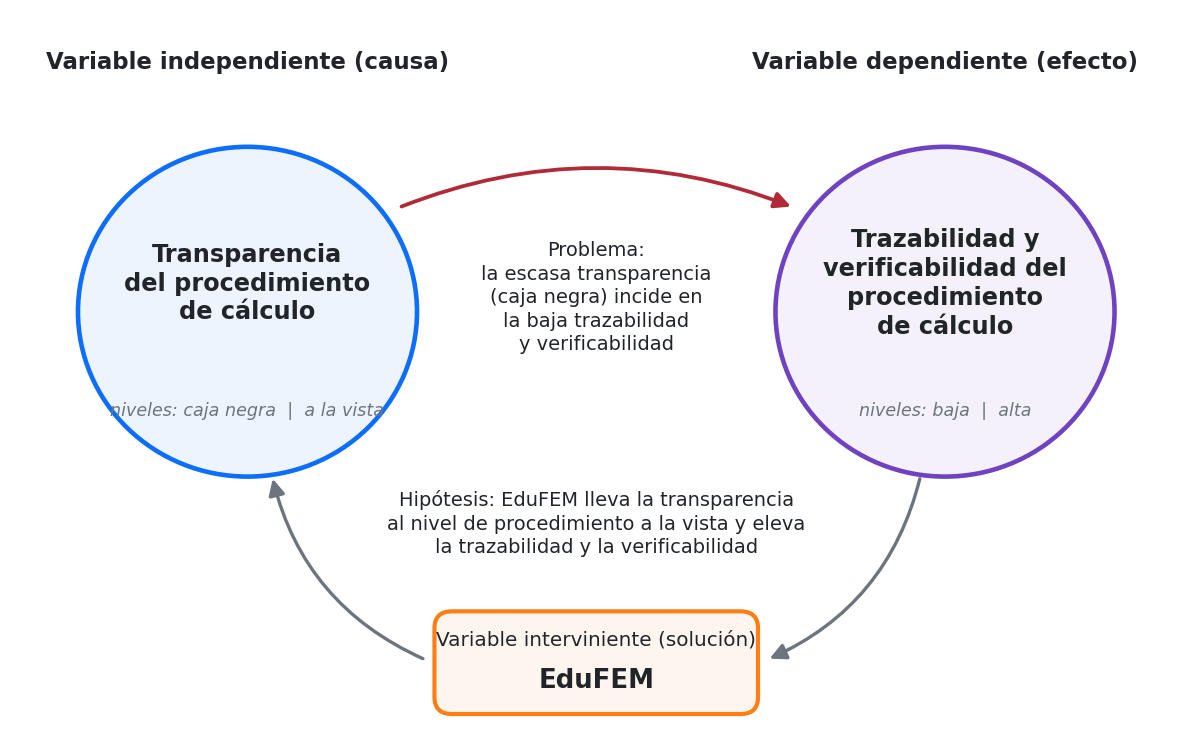
\includegraphics[width=0.78\textwidth]{fig_relacion_variables}
\caption{La Figura 2.1 de final3: la relación entre las variables, en el esquema de círculos de las láminas PP 9 y PP 15.}
\end{figure}

\begin{figure}[htbp]
\centering
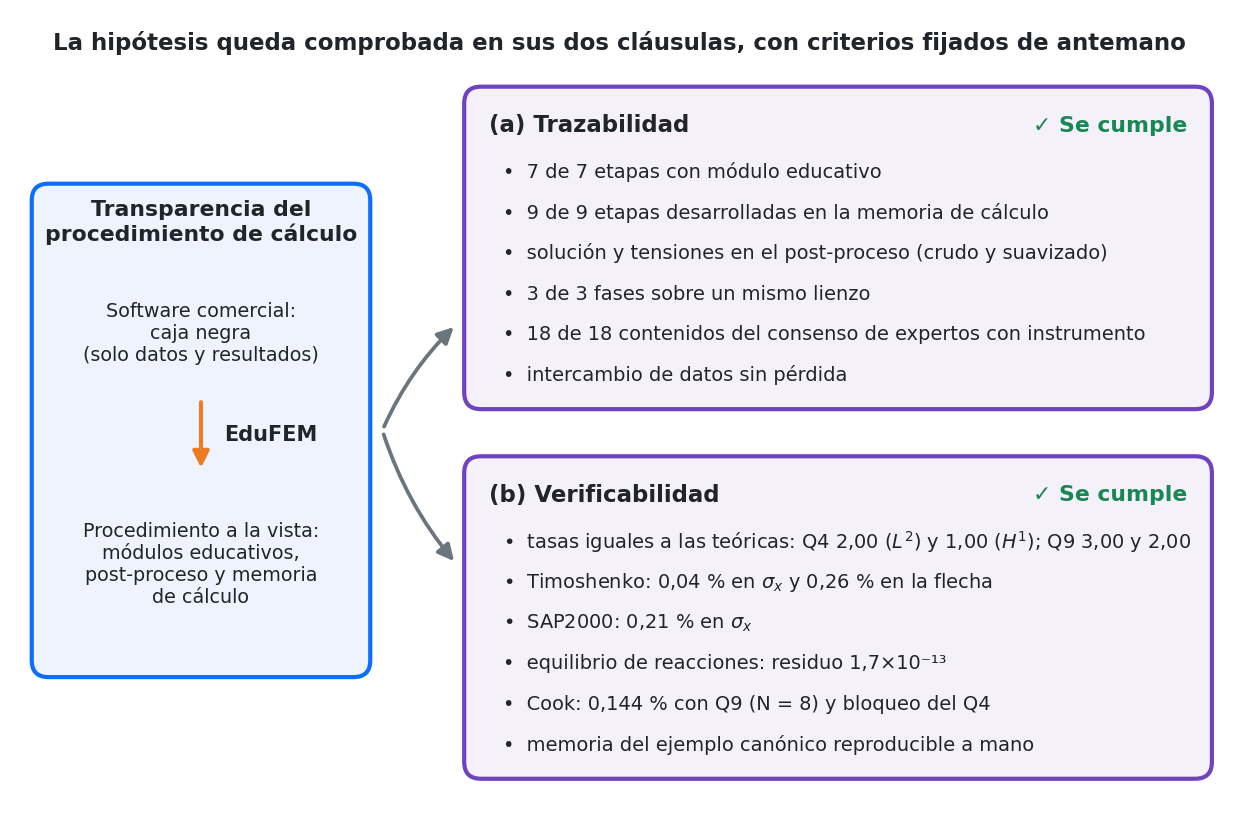
\includegraphics[width=0.86\textwidth]{fig_contraste_hipotesis}
\caption{La Figura CR.1 de final3: el contraste de la hipótesis que abre las Conclusiones.}
\label{fig:cr1}
\end{figure}

\section{Si el Ing.\ Miranda pregunta}

\textbf{«¿Por qué \emph{escasa} y no \emph{nula}?»} Porque la propia tesis registra «Baja (caja negra)» para el software comercial en la Tabla 1.1, y porque ED-Elas2D sí expone las matrices. Con «nula», bastaría un contraejemplo para refutar el problema; con «escasa», el problema describe lo que la tesis documenta.

\textbf{«¿Por qué no \emph{¿Cómo\ldots{} genera\ldots?}»} Porque esa pregunta da la respuesta por supuesta. Su propia lámina de redacción del problema (PP 10) usa \emph{«¿De qué manera\ldots{} podrá afectar en\ldots?»}, y la tesis la sigue con «podrá incidir en».

\textbf{«¿Por qué tres objetivos y no cuatro, como en el Caso II?»} Porque así cada objetivo da nombre a su capítulo, como él pidió, y la tríada queda uno a uno: tres capítulos, tres conclusiones, tres recomendaciones. El Caso II literal obligaría a llevar la verificación al Capítulo 2 y a partir la evidencia de la verificabilidad.

\textbf{«¿Dónde quedó el diagnóstico?»} En la fundamentación. Es documental ---los antecedentes y la Tabla 1.1--- y de él salen los cinco requisitos. Una tesis de grado no lleva diagnóstico de campo (su lámina OG 13, Caso I).

\textbf{«Si el procedimiento es transparente, ¿no es trazable por definición?»} No. Exponer las etapas no asegura que la cadena esté completa sobre el modelo del usuario (trazabilidad) ni que lo expuesto sea correcto (verificabilidad). El ejemplo está en la tesis: el defecto en la matriz de extrapolación del Q4 estaba a la vista y era incorrecto. Lo delató la memoria de cálculo, no las normas de error (§3.7.2).

\textbf{«¿Por qué la universidad solo aparece en la delimitación?»} Porque la tesis mide el software, no a la Carrera; la Carrera es el destino de la herramienta. Es lo que él mismo pidió al decir que el documento es general.

\section{Lo que queda para el autor}

\begin{itemize}
    \item \textbf{Revisar el PDF de final3} (\texttt{tesis/main\_final3.pdf}). Mirar sobre todo la Introducción, la Figura 2.1, la matriz de consistencia (§2.1.3) y las Conclusiones.
    \item \textbf{Confirmar con el Reglamento de Graduación} (H-1) el interlineado y los márgenes. Hoy siguen APA: doble espacio y 2,54~cm.
    \item \textbf{Presentación y video de defensa:} siguen \texttt{main\_final.tex}, y ponerlos al día con final3 es otra tarea (nuevos problema, objetivos, hipótesis y títulos; láminas de conclusiones con la tríada).
    \item \textbf{Retiro de PyMuPDF:} final3 recoge el cambio que otra sesión hizo en el software y en final2 el mismo día. La revisión del instalador queda pendiente de commit (hay un \texttt{\% DATO PENDIENTE} con su hash en el §2.1.1).
    \item Siguen abiertas, sin cambios, la decisión del MMS ($\lambda$ y $D_{33}$) y las demás que registra \url{docs/notas/ESTADO.md}.
\end{itemize}

\end{document}
